\label{sec:general_setting}
%\vspace{-0.5em}
This setting generalizes all the special cases. 
%The pseudo-code is given in Algorithm \ref{alg:five} builds upon the ideas developed for each of the special cases.
%We  require additional notation. 
For each offline dataset $j \in [K]$ and stationary segment of the online stream $k \in [H_T]$, denote by  $\Delta^{(j;k)} = \text{Shift}(f_{(j)}, f^{(k)},p)$, where $f_{(j)}$ is the distribution of offline dataset $j$ and $f^{(k)}$ the distribution of the $k$th online segment (Def. \ref{def:piecewise}). Identical to Theorem \ref{thm:online_shift}, for each $k \in [H_T]$,  $\Delta_k =  \text{Shift} (f^{(k)},f^{(k-1)},p)$ is the shift between the $k$th and $k-1$th online segment. Similar to Theorem \ref{thm:setting_3}, for each $k \in [H_T]$ and offline dataset $j \in [K]$,  $\widehat{\tau}_j^{(k)} = \inf \{ \widehat{\tau}: 3(u_{\widehat{\tau}}(\alpha) + u_{N_j}(\alpha)) \leq \text{Shift}(f^{(k)},f_{(j)},p) \}$, where $\widehat{\tau}_j^{(k)} = \infty$ if $\text{Shift}(f^{(k)},f_{(j)},p)=0$.  Assumption \ref{defn:offline_datasets} guarantees $\text{Shift}(f^{(k)},f_{(j)},p)>0\implies\widehat{\tau}_j^{(k)}  < \infty$. Similar to Eq. (\ref{eqn:defn_tau_hat}),  $\widehat{\tau}^{(k)} = \max \{ \lceil \widehat{\tau}_j^{(k)} \rceil \text{ : } \widehat{\tau}_j^{(k)}  < \infty \}.$
% is finite independent of $T$.%Given a piecewise-stationary stream $(S_t)_{t=1}^T$ and the $K$ offline datasets, for each segment $k \in [H_T]$, denote by 
\begin{equation}
    \widetilde{D}_k(\alpha) = D(\Delta_k,\alpha) + \widehat{\tau}^{(k)}.
    \label{eqn:D_tilde}
\end{equation}

In words, $\widetilde{D}_k(\alpha)$ is the \emph{worst-case} delay after the $k$th change point has occurred on the data-stream for Algorithm \ref{alg:five} to both {\em(i)} detect that the online stream has undergone a shift, and {\em(ii)} identify if any of the offline datasets' $p$th quantile matches the new $p$th quantile. 


\begin{algorithm}[h!]
\caption{General thresholding algorithm}\label{alg:five}
\SetKwInOut{Input}{Input}
\SetKwInOut{Output}{Output}
\Input{ $p, \alpha \in (0,1)$, offline datasets $\gD_1, \gD_2, \ldots, \gD_K$. }
\Output{Anomaly labels $\hat{y}_1, \hat{y}_2, \ldots$}
$\tau \gets 0$  \tcp*{\small{previous change point}}
% \For{$j = 1, \ldots, K$}{
%         $CS_{j\text{forward}} \gets C(p,\alpha,\gD_j)$\;
%         }
\For{ $\text{each time }t \geq 1$ } {
    Receive $t^{th}$ input $S_t$\;
    
    % $CS_{\text{online}} \gets C(p,\alpha, S_{\tau:t})$  \;
    % $CS_{\text{backward}} \gets CS(\{S_i\}_{i=\tau}^{t})$\;
    % \tcp{\small{detect shift}}
    \uIf{{\ttfamily Algorithm-}\ref{alg:change_point} $(p,\alpha,S_{\tau+1:t-1})==1$}{
        $\hat{y}_t \gets * $ \; \tcp{Change-point detected}
        $\tau \gets t-1$ \;
    } \Else {
    $\hat{y}_t \gets \text{{\ttfamily Algorithm-}\ref{alg:decision_making_datasets}} (p,\alpha, S_{\tau+1:t-1}, (\gD_{1:K}))$
  %   \tcp{\small{Check for matching datasets}}
  %   % \For{$j = 1, \ldots, k$}{
  %   %     $\text{m}_j \gets $ \small{$\mathbf{1}(CS_{j\text{forward}-t} \cap CS_{\text{backward}-t} \neq \emptyset)$}\;
  %   % }
  %   m = $\Sigma_j \mathbf{1}(CS_{j\text{forward}-t} \cap CS_{\text{backward}-t} \neq \emptyset)$\;
  %   \uIf{$m =1 $}{
  %       $\hat{y}_t \gets $  \small{Algo-\ref{alg:one} $(p, 1-\alpha, \gD_{j\text{match}}  \cup \{S_{\tau},  \ldots , S_t\})$}\;
  %   }
  %   \Else{
  %       \tcp{\small{use online estimation}}
  %       $\hat{y}_t \gets$  \small{Algo-\ref{alg:one} $(p, 1-\alpha, \{S_{\tau},  \ldots , S_t\})$}\;
  % }
  }
}
\end{algorithm}

% \begin{algorithm}[h!]
% \caption{General thresholding algorithm}\label{alg:five}
% \SetKwInOut{Input}{Input}
% \SetKwInOut{Output}{Output}
% \Input{Quantile $p$, Confidence $1-\alpha$, offline datasets $\gD_1, \gD_2, \ldots, \gD_K$. }
% \Output{Anomaly labels $\hat{y}_1, \hat{y}_2, \ldots$}
% $\tau \gets 0$  \tcp*{\small{previous change point}}
% \For{$j = 1, \ldots, K$}{
%         $CS_{j\text{forward}} \gets C(p,\alpha,\gD_j)$\;
%         }
% \For{ $\text{each time }t \geq 1$ } {
%     Receive $t^{th}$ input $S_t$\;
    
%     $CS_{\text{online}} \gets C(p,\alpha, S_{\tau:t})$  \;
%     $CS_{\text{backward}} \gets CS(\{S_i\}_{i=\tau}^{t})$\;
%     \tcp{\small{detect shift}}
%     \uIf{$CS_{\text{online}-i }\cap CS_{\text{backward}-(t-\tau-i)} = \emptyset$ for any $i \in [1, t-\tau]$}{
%         $\hat{y}_t \gets * $ \;
%         $\tau \gets t$ \;
%     } \Else {
%     \tcp{\small{Check for matching datasets}}
%     % \For{$j = 1, \ldots, k$}{
%     %     $\text{m}_j \gets $ \small{$\mathbf{1}(CS_{j\text{forward}-t} \cap CS_{\text{backward}-t} \neq \emptyset)$}\;
%     % }
%     m = $\Sigma_j \mathbf{1}(CS_{j\text{forward}-t} \cap CS_{\text{backward}-t} \neq \emptyset)$\;
%     \uIf{$m =1 $}{
%         $\hat{y}_t \gets $  \small{Algo-\ref{alg:one} $(p, 1-\alpha, \gD_{j\text{match}}  \cup \{S_{\tau},  \ldots , S_t\})$}\;
%     }
%     \Else{
%         \tcp{\small{use online estimation}}
%         $\hat{y}_t \gets$  \small{Algo-\ref{alg:one} $(p, 1-\alpha, \{S_{\tau},  \ldots , S_t\})$}\;
%   }
%   }
% }
% \end{algorithm}

% To state performance guarantee of Algorithm \ref{alg:five}, we need a definition of a good event, which occurs with high probability.
% \begin{definition}[Good event 4] 
% Given a piece-wise stationary sequence $(S_t)_{t=1}^T := \Bigl(T,H_T, (\tau_c)_{c=0}^{H_T}, (f^{(c)})_{c=0}^{H_T}\Bigr)$, with the quantile functions of the $H_T+1$ different segments given by $(Q^{(c)}(\cdot))_{c=1}^{H_T}$ and $K$ offline datasets that are $(p,\alpha)$ separated according to Definition \ref{defn:offline_datasets}, let
% \begin{align}
% \begin{split}
%     \gE_4 = \underbrace{\bigcap_{l=1}^{K}\bigg\{ Q_{(l)}(p) \in C(p,\alpha, \{X_j^{(l)}\}_{j=1}^{N_l}) \bigg\}}_{\text{Offline dataset's CS contain true quantile}}   \\ \underbrace{\bigcap_{k=0}^{H_T} \bigcap_{t_1 = \tau_{k}}^{\tau_{k+1}} \bigcap_{t_2 = t_1 + 1}^{\tau_{k+1}}   \{ Q^{(k)}(p) \in C(p,\alpha,S_{t_1:t_2}) \}}_{\text{Online stream's CS contain true quantile}},
%         \end{split}
%                 \label{eqn:good_event_4_defn}
% \end{align}
% where the $p$th quantile of the offline datasets $Q_{(l)}(p)$ are defined in Definition \ref{def:offline_quantile}.
% \end{definition}
% \vspace{-0.5em}
% %
% Event $\gE_4$ is the union of $\gE_2$ in equation \ref{eqn:good_event_2_defn} for the online stream along with the event $\gE_3$ in Equation (\ref{eqn:good_event_3}) for the offline datasets. A union bound implies that the event $\mathbb{P}[\gE_4] \geq 1- \alpha (K+T)$. 

%The main result of this paper is stated below.




%The main result of t

\begin{theorem}[\textbf{Main result of Algorithm \ref{alg:five}}] For a desired $\alpha \in (0,1)$, suppose the piece-wise stationary online stream $(S_t)_{t=1}^T \sim \Bigl(T,H_T, (\tau_c)_{c=0}^{H_T}, (f_c)_{c=0}^{H_T}\Bigr)$ is $\alpha$-detectable, i.e., satisfies Assumption \ref{asumption_detectable}, and the offline datasets  $\gD_1, \ldots, \gD_K$ are $(p,\alpha)$-separated according to Definition \ref{defn:offline_datasets}. %Denote by the online quantile shifts as $\Delta_{k} = \text{Shift} (f^{(k)},f^{(k-1)},p)$ for $k \in [H_T]$. 
Then, for all times $T \in \mathbb{N}$, with probability at-least $1-(K+2T)\alpha$,  Algorithm \ref{alg:five} satisfies \emph{both},
%{\em (i)} $\text{FP} + \text{FN}  \leq \sum_{k=1}^{H_T} \widetilde{D}_k(\alpha)$, and {\em(ii)} Abstains $\leq \sum_{k=1}^{H_T} \Bigl[ (1-\mathbf{1}_{\text{Match}_k}) \mathcal{O}(\sqrt{\tau_k - \tau_{k-1}}) \footnote{Constants are in the Appendix and report here the order-wise result to highlight the main terms in the bound. } + \mathbf{1}_{\text{Match}_k}\left(\gO(\sqrt{N^{(k)}+(\tau_k-\tau_{k-1})} - \sqrt{N^{(k)}}) \right) +  \widetilde{D}_k(\alpha) \Bigr]$,
\begin{itemize}
    \item  $\text{FP} + \text{FN}  \leq \sum_{k=1}^{H_T} D(\Delta_k,\alpha) + (1-\mathbf{1}_{\text{Match}_k})\max_{ j \in [K]} \left(\lceil \widehat{\tau}_j^{(k)}\rceil \mathbf{1}_{\text{Shift}(f^{(k)},f_{(j)},p) > 0}\right)$ 
     \item Abstains $ \leq \sum_{k=1}^{H_T} \Bigl[ (1-\mathbf{1}_{\text{Match}_k}) \mathcal{O}(\sqrt{\tau_k - \tau_{k-1}}) \footnote{Constants are in the Appendix and report here the order-wise result to highlight the main terms in the bound. } +  \mathbf{1}_{\text{Match}_k}\left(\gO(\sqrt{N^{(k)}+(\tau_k-\tau_{k-1})} - \sqrt{N^{(k)}}) \right) +  \widetilde{D}_k(\alpha) \Bigr]$
 \end{itemize}
where $\mathbf{1}_{\text{Match}_k} = \mathbf{1}_{Q^{(k)}(p) \in \{Q_{(1)}(p), \cdots, Q_{(K)}(p)\}}$, and $Q^{(k)}(p)$ is the $p$th quantile of the $k$th segment of the online stream (Def. \ref{def:piecewise}), $Q_{(1)}(p), \cdots, Q_{(K)}(p)$ are the $p$th quantiles of the offline datasets (Definition \ref{definition:offline_dataset}),   $N^{(k)} = \min \{N_j: Q_{(j)}(p) = Q^{(k)}(p)\}$ and $\widetilde{D}_k(\alpha)$ is defined in Equation (\ref{eqn:D_tilde}). 
\label{thm:core_theorem}
\end{theorem}

Observe that Theorem \ref{thm:core_theorem} recovers Theorem \ref{thm:setting_3}  if $(S_t)_{t\geq 1}$ is i.i.d. Theorem \ref{thm:core_theorem} shows that even in the general case,  $\text{FP} + \text{FN}$ only scale with the number and complexity of change-points, and not with the stream length $T$. 
%The term $\widetilde{D}_k(\alpha)$ for each $k \in [H_T]$ in Equation (\ref{eqn:D_tilde}) is the delay incurred in both detecting the $k$th change-point and deciding which if any of the offline dataset's $p$th quantile matches the $k$th stationary segment.
% We now read off several remarks from Theorem \ref{thm:core_theorem}.


\begin{figure}
\centering
\begin{subfigure}{.48\columnwidth}
  \centering
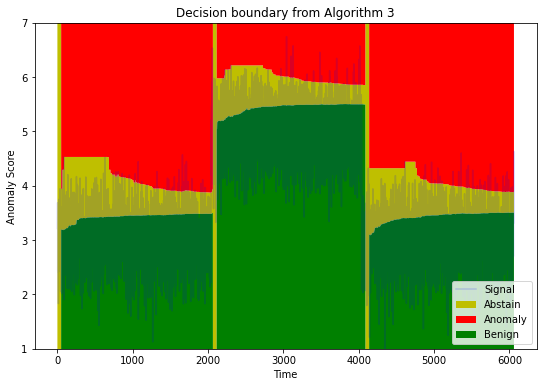
\includegraphics[width=\linewidth]{anomaly/figs/4-2.png}
  %\caption{A subfigure}
  \caption{}
  \label{fig:s41}
\end{subfigure}%
\begin{subfigure}{.48\columnwidth}
  \centering
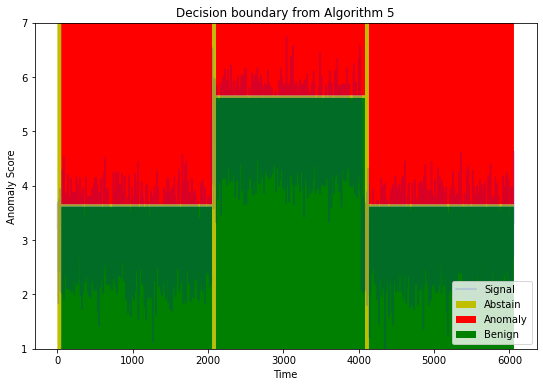
\includegraphics[width=\linewidth]{anomaly/figs/4-1.png}
  %\caption{Anomaly threshold set using a fixed cold-start period}
  \caption{}
  \label{fig:s42}
\end{subfigure}%
\vspace{-0.5em}
\caption{Decision boundaries for the same synthetic data stream, without offline dataset $(a)$ and with $(b)$. Incorporating datasets allows us to significantly reduce abstention.}\vspace{-2em}
\label{fig:s4_example}
\end{figure}
%\vspace{-4em}

%\textbf{Mistakes do not scale with $T$.}
   
% \begin{itemize}
%     \item Case $\Delta = 0$:
%     \begin{itemize}
%         \item $FP= 0$, $FN=0$
%         \item Abstains $= 4 \sqrt{(N+T) \ln \left( \frac{1612\ln(e(N+T))}{\alpha^2} \right)}- 4 \sqrt{N \ln \left( \frac{1612\ln(eN)}{\alpha^2} \right)}$
%     \end{itemize}
%     \item Case  $\Delta > 0$:
%     \begin{itemize}
%         \item $FP+FN \leq D(\Delta,\alpha) $
%         \item Abstains $\leq D(\Delta,\alpha) + 4 \sqrt{T \ln \left( \frac{1612\ln(eT)}{\alpha^2} \right)}$
%     \end{itemize}
% \end{itemize}

%We show in Corollary \ref{cor:general_flex_1} that when the offline datasets when, abstains are reduced (see also Figure \ref{fig:s4_example}).

\textbf{Abstains reduced if offline data is useful.}
     Suppose the online stream $(S_t)_{t=1}^T$  and the offline datasets  $\gD_{1}, \ldots, \gD_K$ are such that for all segments $k \in [H_T]$, there exists an offline dataset $j \in [K]$ s.t. $Q^{(k)}(p) = Q_{(j)}(p)$. Theorem \ref{thm:core_theorem} guarantees that  abstains $\leq \mathcal{O}\left(\sqrt{H_T N} \left(\sqrt{1+\frac{T}{N}} - 1 \right)\right) + \sum_{k=1}^{H_T}\widetilde{D}_k( \alpha)$, where $N = \min \{N_j \text{ : } \exists k \in [H_T] \text{ : } Q_{(j)}(p) = Q^{(k)}(p) \}  $ is size of the smallest useful offline dataset. Thus, if the useful offline data is large ($N >> T$), the fraction of abstains is small even in the presence of non-stationarity (Fig. \ref{fig:s4_example} ). 
     %\label{cor:general_flex_1}
     
%Corollary \ref{cor:general_flex_1} shows that in the worst-case when the offline distribution can be arbitrary, the performance degradation is bounded. 

\textbf{Bounded degradation if offline data is arbitrary.}
Theorem \ref{thm:core_theorem} proves that in the worst-case when the offline datasets are arbitrary, abstains are at-most $ \mathcal{O}(\sqrt{H_T T}) + \sum_{k=1}^{H_T}\widetilde{D}_k(\alpha)$, which is comparable to Theorem \ref{thm:online_shift}, with an additional additive term of $\sum_{k=1}^{H_T}\widetilde{D}_k(\alpha)$. This extra term arises due to incurring delay in both identifying a change-point on the online stream, and deciding that either the new segment has the same $p$th quantile as one of the offline datasets or not. This penalty is incurred since Algorithm \ref{alg:five} does not know both the time of change-points and if the $p$th quantile of any offline datasets equals that of the online. Thus, Theorem \ref{thm:core_theorem} is adaptive, yielding low mistakes and abstains in the event that the offline dataset is useful while simultaneously bounding worst-case performance independent of $T$ and $N$ when the offline dataset is arbitrary. 


     %For a desired $\alpha \in (0,1)$, suppose the online stream $(S_t)_{t=1}^T$ satisfy the conditions in Theorem \ref{thm:core_theorem}  and the offline datasets  $\gD_{1}, \ldots, \gD_K$ satisfy Assumption \ref{as:offline_detectable}, but are otherwise arbitrary. Then, with probability at-least $1- (K+T)\alpha$, 
     %\label{cor:general_flex_2}

%Corollary \ref{cor:general_flex_2} shows that in the worst case when the offline distributions are arbitrary, the number of abstains  %Moreover, the worst case bound is independent of stream length $T$ and offline dataset size $N$. 

% \begin{remark}[Best case scenario for Algorithm \ref{alg:five}] Even though the worst case bounds of Theorem \ref{thm:core_theorem} is the same as that of Theorem \ref{thm:online_shift} (online distribution shift setting), we can apply the analysis of Theorem \ref{thm:setting_3} (stationary + dataset setting) on each stationary piece of the stream. If all of the pieces match the offline datasets, the number of abstains is reduced to be less than $ \sum_{k=1}^{H_t} \left( D(\Delta_k,\alpha) + \gO(\sqrt{N+(\tau_k-\tau_{k-1})} - \sqrt{N})\right) $. 
% \end{remark}




%\abishek{Add flex of how this result is proved.}
